\begin{frame}[fragile]{Schema del database World}
\begin{figure}
    \centering
        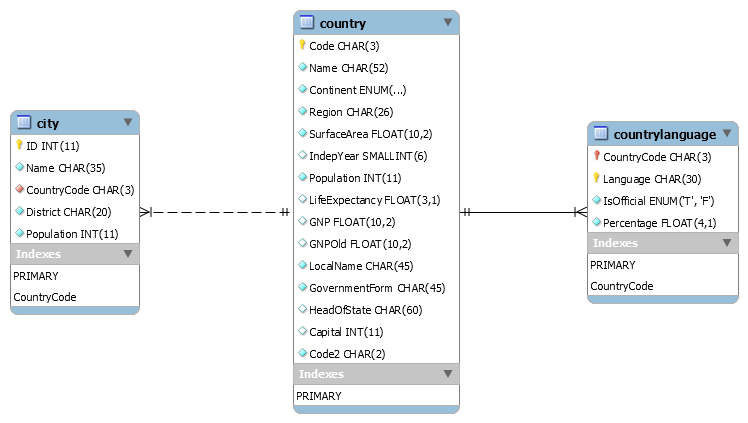
\includegraphics[width=.8\textwidth]{img/db-world.png}
    \end{figure}
\end{frame}
%
\begin{frame}[fragile]{World: Es. 1}
Visualizzare id, nome, popolazione dalla tabella \textit{city} e limitare i risultati solo alle prime 10 righe.
\pause
\begin{lstlisting}
SELECT Id, Name, Population
FROM city
LIMIT 10;
\end{lstlisting}
\end{frame}
%
\begin{frame}[fragile]{World: Es. 2}
Visualizzare id, nome, popolazione dalla tabella \textit{city} e limitare i risultati alle righe 31-40.
\pause
\begin{lstlisting}
SELECT Id, Name, Population
FROM city
LIMIT 30, 10;
\end{lstlisting}
\end{frame}
%
\begin{frame}[fragile]{World: Es. 3}
Trovare dalla tabella \textit{city} solo le citt\`a la cui popolazione \`e superiore a 2000000.
\pause
\begin{lstlisting}
SELECT Name, Population
FROM city
WHERE Population > 2000000;
\end{lstlisting}
\end{frame}

%
\begin{frame}[fragile]{World: Es. 4}
Trovare tutti i nomi di citt\`a dalla tabella \textit{city} il cui nome inizia con il prefisso 'Be'.
\pause
\begin{lstlisting}
SELECT Name
FROM city
WHERE Name LIKE 'Be%';
\end{lstlisting}
In questo modo non viene fatto nessun controllo per le lettere accentate.
\end{frame}

\begin{frame}[fragile]{World: Es. 4}
Trovare tutti i nomi di citt\`a dalla tabella \textit{city} il cui nome inizia con il prefisso 'Be'.
\begin{lstlisting}
SELECT Name
FROM city
WHERE Name LIKE 'Be%' COLLATE utf8mb4_bin;
\end{lstlisting}
\textbf{COLLATE} = clausola per indicare quale collazione utilizzare con la clausola precedente.
\newline
\newline
Collazione = insieme di regole che influiscono su come i dati alfanumerici vengono confrontati, ordinati e ricercati.
\end{frame}

%
\begin{frame}[fragile]{World: Es. 5}
Trovare dalla tabella \textit{city} solo le citt\`a la cui popolazione \`e compresa tra 500000 e 1000000.
\pause
\begin{lstlisting}
SELECT Name, Population
FROM city
WHERE Population BETWEEN 500000 AND 1000000;
\end{lstlisting}
\pause
oppure
\begin{lstlisting}
SELECT Name, Population
FROM city
WHERE Population >= 500000 AND Population <=1000000;
\end{lstlisting}
\end{frame}
%
\begin{frame}[fragile]{World: Es. 6}
Visualizzare tutte le citt\`a della tabella \textit{city} ordinate per nome in ordine crescente.
\pause
\begin{lstlisting}
SELECT *
FROM city
ORDER BY Name ASC;
\end{lstlisting}
oppure
\pause
\begin{lstlisting}
SELECT *
FROM city
ORDER BY Name;
\end{lstlisting}
\end{frame}
%
\begin{frame}[fragile]{World: Es. 7}
Trovare la citt\`a con la popolazione pi\`u bassa nella tabella \textit{city}.
\pause
\vspace{-.1cm}
\begin{lstlisting}
SELECT Name
FROM city
WHERE population = (
    SELECT MIN(Population)
    FROM city
);
\end{lstlisting}
\end{frame}
%
\begin{frame}[fragile]{World: Es. 7}
Trovare la citt\`a con la popolazione pi\`u bassa nella tabella \textit{city}.

Altra possibile soluzione:
\vspace{-.1cm}
\begin{lstlisting}
SELECT Population, Name
FROM city
WHERE Population IS NOT NULL
ORDER BY Population ASC
LIMIT 1;
\end{lstlisting}
\end{frame}
%
\begin{frame}[fragile]{World: Es. 8}
Trovare la citt\`a con la popolazione pi\`u bassa nella tabella \textit{country}.
\pause
\\Prima troviamo la \textbf{popolazione pi\`u bassa}:
\begin{lstlisting}
SELECT MIN(Population)
FROM country;
\end{lstlisting}
\pause
Poi facciamo una \textbf{query annidata} dove cerchiamo tutte le citt\`a che hanno poplazione = a quella appena trovata:
\begin{lstlisting}
SELECT Name, Population
FROM country
WHERE Population = (
    SELECT MIN(Population)
    FROM country
);
\end{lstlisting}
\end{frame}
%
\begin{frame}[fragile]{World: Es. 9}
Trovare il paese con la popolazione pi\`u numerosa nella tabella \textit{country}.
\pause
\begin{lstlisting}
SELECT Population, Name
FROM country
WHERE Population IS NOT NULL
ORDER BY Population DESC
LIMIT 1;
\end{lstlisting}
\end{frame}
%
\begin{frame}[fragile]{World: Es. 9}
Trovare il paese con la popolazione pi\`u numerosa nella tabella \textit{country}.

Altra soluzione possibile:
\pause
\\Prima troviamo la \textbf{pi\`u alta aspettativa di vita}:
\begin{lstlisting}
SELECT MAX(Population)
FROM country;
\end{lstlisting}
\pause
Poi facciamo una \textbf{query annidata} dove cerchiamo tutte le citt\`a che hanno come popolazione quella appena trovata:
\begin{lstlisting}
SELECT Population, Name
FROM country
WHERE Population = (
    SELECT MAX(Population)
    FROM country
);
\end{lstlisting}
\end{frame}
%
\begin{frame}[fragile]{World: Es. 10}
Elencare tutte le lingue parlate nella regione dei Caraibi (`Caribbean'). 
\pause
\begin{lstlisting}
SELECT DISTINCT country.Region, countrylanguage.Language
FROM country LEFT JOIN countrylanguage
ON country.Code = countrylanguage.CountryCode
WHERE country.Region = `Caribbean';
\end{lstlisting}
\end{frame}
%
\begin{frame}[fragile]{World: Es. 11}
Trovare la capitale della Spagna (ESP).
\pause
\begin{lstlisting}
SELECT city.Name
FROM city JOIN country ON city.ID = country.Capital
WHERE city.CountryCode = `ESP';
\end{lstlisting}
\end{frame}
%
\begin{frame}[fragile]{World: Es. 12}
Trovare il paese con la pi\`u alta aspettativa di vita.
\pause
\begin{lstlisting}
SELECT country.Name, LifeExpectancy
FROM country
ORDER BY LifeExpectancy DESC
LIMIT 1;
\end{lstlisting}
\end{frame}
%
\begin{frame}[fragile]{World: Es. 12}
Trovare il paese con la pi\`u alta aspettativa di vita.

Altra soluzione Possibile:
\pause
\\Prima troviamo la \textbf{pi\`u alta aspettativa di vita}:
\begin{lstlisting}
SELECT MAX(LifeExpectancy)
FROM country;
\end{lstlisting}
\pause
Poi facciamo una \textbf{query annidata} dove cerchiamo quell'aspettativa di vita appena trovata:
\begin{lstlisting}
SELECT country.Name, LifeExpectancy
FROM country
WHERE LifeExpectancy = (
    SELECT MAX(LifeExpectancy)
    FROM country
);
\end{lstlisting}
\end{frame}
%
\begin{frame}[fragile]{World: Es. 13}
Trovare tutte le citt\`a del continente europeo.
\pause
\begin{lstlisting}
SELECT city.Name
FROM city JOIN country ON city.CountryCode = country.Code
WHERE country.Continent = `Europe';
\end{lstlisting}
\end{frame}
%
\begin{frame}[fragile]{World: Es. 14}
Aggiornare il presidente degli Stati Uniti attualmente presente sul database, con `Donald Trump'.
\pause
\begin{lstlisting}
UPDATE country
SET HeadOfState = `Donald Trump'
WHERE Code = `USA';
\end{lstlisting}
\end{frame}
%

\begin{comment}    

\begin{frame}[fragile]{World: Es. 15}
Trovare la citt\`a pi\`u popolata nella tabella \textit{city}.
\pause
\newline
\\Stesso ragionamento delle query precedenti (query annidata):
\begin{lstlisting}
SELECT Name, Population
FROM city
WHERE Population = (
    SELECT MAX(Population)
    FROM city
);
\end{lstlisting}
\end{frame}
%
\begin{frame}[fragile]{World: Es. 16}
Trovare la citt\`a meno popolata nella tabella \textit{city}.
\pause
\newline
\\Stesso ragionamento delle query precedenti (query annidata):
\begin{lstlisting}
SELECT Name, Population
FROM city
WHERE Population = (
    SELECT MIN(Population)
    FROM city
);
\end{lstlisting}
\end{frame}
%
\begin{frame}[fragile]{World: Es. 17}
Calcolare il numero di record della tabella \textit{city}.
\pause
\begin{lstlisting}
SELECT COUNT(Id) AS `n. di citta'
FROM city;
\end{lstlisting}
\end{frame}
%

\end{comment}


\begin{frame}[fragile]{World: Es. 15}
Ottenere il numero di citt\`a in Cina dalla tabella \textit{city}.

La Cina ha country code 'CHN'.
\pause
\begin{lstlisting}
SELECT COUNT(*)
FROM city
WHERE CountryCode = 'CHN';
\end{lstlisting}
\end{frame}
%

\begin{frame}[fragile]{World: Es. 16}
Crea una copia della tabella \textit{city}.
La struttura deve essere la stessa, per\`o deve contenere solo le citt\`a con poplazione superiore a 5000000.
\pause
\begin{lstlisting}
CREATE TABLE big_cities AS 
SELECT *
FROM city
WHERE city.Population > 5000000;
\end{lstlisting}
Questa soluzione pu\`o portare ad errori, in quanto la nuova tabella non eredita definizioni come l'auto-incremento.
\end{frame}


\begin{frame}[fragile]{World: Es. 16}
Crea una copia della tabella \textit{city}.
La struttura deve essere la stessa, per\`o deve contenere solo le citt\`a con poplazione superiore a 5000000.
\begin{lstlisting}
CREATE TABLE big_cities LIKE city;

INSERT INTO big_cities
SELECT *
FROM city
WHERE city.Population > 5000000;
\end{lstlisting}
Grazie alla clausola LIKE la tabella eredita tutte le definizioni.
\end{frame}
%

\begin{frame}[fragile]{World: Es. 17}
Elenca i paesi che hanno almeno due lingue ufficiali. Mostra il nome del paese e il numero di lingue ufficiali.
\pause
\begin{lstlisting}
SELECT c.Name, COUNT(*) AS num_lingue
FROM country AS c
JOIN countrylanguage AS cl
ON c.Code = cl.CountryCode
WHERE cl.IsOfficial = 'T'
GROUP BY c.Code
HAVING num_lingue >= 2;
\end{lstlisting}
\end{frame}
%

\begin{frame}[fragile]{World: Es. 18}
Mostra le prime 5 lingue non ufficiali pi\`u parlate nel mondo in base alla somma delle 
popolazioni dei paesi in cui sono parlate. Indica la lingua e la popolazione totale.
\pause
\begin{lstlisting}
SELECT cl.Language, 
    SUM(c.Population * cl.Percentage / 100) 
    AS num_population
FROM country AS c JOIN countrylanguage AS cl 
    ON c.Code = cl.CountryCode
WHERE cl.IsOfficial = 'F'
GROUP BY cl.Language
ORDER BY num_population DESC
LIMIT 5;
\end{lstlisting}
\end{frame}
%

\begin{frame}[fragile]{World: Es. 19}
Trova tutti i paesi in cui si parla almeno una delle due tra inglese ('English') e francese ('French'). 
Mostra il nome del paese e la lingua.
USARE GLI OPERATORI INSIEMISTICI.
\pause
\begin{lstlisting}
SELECT country.Name, countrylanguage.Language
FROM country
JOIN countrylanguage 
    ON country.Code = countrylanguage.CountryCode
WHERE countrylanguage.Language = 'English'
UNION
SELECT country.Name, countrylanguage.Language
FROM country
JOIN countrylanguage 
    ON country.Code = countrylanguage.CountryCode
WHERE countrylanguage.Language = 'French';
\end{lstlisting}
\end{frame}
%

\begin{frame}[fragile]{World: Es. 20}
Trova tutti i paesi in cui si parla almeno una lingua non ufficiale.
\pause
\begin{lstlisting}
SELECT c.Name
FROM country AS c
JOIN countrylanguage AS cl on c.Code = cl.CountryCode
WHERE cl.IsOfficial = 'F'
GROUP BY c.Code
HAVING COUNT(*) >= 1;
\end{lstlisting}
\end{frame}

\begin{frame}[fragile]{World: Es. 20}
Trova tutti i paesi in cui si parla almeno una lingua non ufficiale.
\newline
\newline
Versione con EXIST
\begin{lstlisting}
SELECT c.Name
FROM country AS c
WHERE EXISTS (
    SELECT 1
    FROM countrylanguage AS cl
    WHERE cl.CountryCode = c.Code
        AND cl.IsOfficial = 'F'
);
\end{lstlisting}
\end{frame}

\begin{frame}[fragile]{World: Es. 20}
Trova tutti i paesi in cui si parla almeno una lingua non ufficiale.
\newline
\newline
Versione con IN
\begin{lstlisting}
SELECT Name
FROM country
WHERE Code IN (
    SELECT CountryCode
    FROM countrylanguage
    WHERE IsOfficial = 'F'
);
\end{lstlisting}
\end{frame}
%


\begin{frame}[fragile]{World: Es. 21}
Elenca i paesi che non hanno nessuna citt\`a registrata nella tabella \textit{city}.
\pause
\newline
\newline
Versione con NOT EXIST
\begin{lstlisting}
SELECT c.Name
FROM country c
WHERE NOT EXISTS (
    SELECT 1
    FROM city ci
    WHERE ci.CountryCode = c.Code
);
\end{lstlisting}
\end{frame}

\begin{frame}[fragile]{World: Es. 21}
Elenca i paesi che non hanno nessuna citt\`a registrata nella tabella \textit{city}.
\newline
\newline
Versione con NOT IN
\begin{lstlisting}
SELECT Name
FROM country
WHERE Code NOT IN (
    SELECT CountryCode
    FROM city
);
\end{lstlisting}
\end{frame}

\begin{frame}[fragile]{World: Es. 21}
Elenca i paesi che non hanno nessuna citt\`a registrata nella tabella \textit{city}.
\newline
\newline
Versione con LEFT JOIN
\begin{lstlisting}
SELECT c.Name
FROM country c
LEFT JOIN city ci ON c.Code = ci.CountryCode
WHERE ci.ID IS NULL;
\end{lstlisting}
\end{frame}

